\documentclass{article}

\usepackage[margin=1in]{geometry}
\usepackage{graphicx}
\usepackage{hyperref}
\usepackage{listings}
\usepackage[T1]{fontenc}
\lstset{language=bash, basicstyle=\small\ttfamily, showstringspaces=false}

\begin{document}

\title{Learning git and github for LESGO users}
\date{}

\maketitle

\section{Why do we use git?}
\begin{itemize}
\item Full version history. Did you make a mistake or want to go back and look at previous versions of the code? It's all right there in the repository. This also serves as a kind of backup.
\item Collaboration. Git makes it easy to save changes and share it with others. 
\item Branching. You can work on several new features at the same time using different branches. When you're done, you can easily merge the new feature branch into the main code.
\end{itemize}

\section{Using the fork and pull workflow with Github using the learn-git repository}

\begin{enumerate}
\item Navigate to the main repository \href{https://github.com/lesgo-jhu/learn-git}{https://github.com/lesgo-jhu/learn-git}. Feel free to play around with this repository. It's a playground to learn what you're doing.
\item Fork your own copy of the repository to your account. This will give you a new repository where you can make changes without affecting the main source code used by others.
\begin{figure*}[h!]
\centering
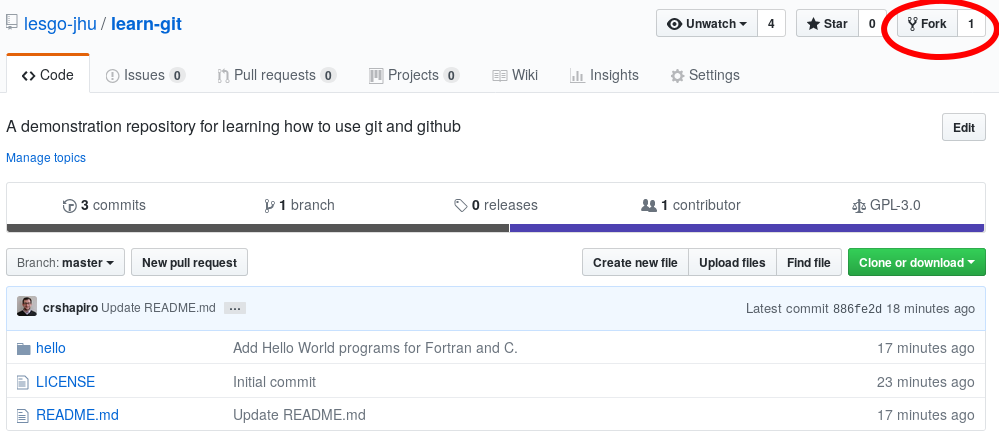
\includegraphics[width=\textwidth]{fork.png}
\end{figure*}
\item Clone your new repository to your local machine, where you will do development
\begin{lstlisting}
git clone https://github.com/crshapiro/learn-git.git
\end{lstlisting}

\item By default, your personal server-side repository is called ``origin.'' We also need to tell git where the official server-side repository is, which we'll call ``upstream.''
\begin{lstlisting}
git remote add upstream https://github.com/lesgo-jhu/learn-git.git
\end{lstlisting}
You can always see the url of ``origin'' and ``upstream'' using
\begin{lstlisting}
git remote show origin
git remote show upstream
\end{lstlisting}

\item Now, we can start making some changes. Write a ``Hello World'' program in your favorite language. Once this is complete, you can commit the changes:
\begin{lstlisting}
git add (list for files)
\end{lstlisting}
To see the status of the added files use:
\begin{lstlisting}
git status
\end{lstlisting}
Now commit the changes to your local repository
\begin{lstlisting}
git commit -m "Enter a concise message detailing changes."
\end{lstlisting}

\item The edits you have made are still only on your local machine. To copy the changes to your server-side repository (origin) use
\begin{lstlisting}
git push 
\end{lstlisting}
This will push to the first remote repository listed in \texttt{git remote}.

Starting August 2021, performing HTTPS git operations on command line also require authentication using a \emph{personal access token (PAT)}.
Follow the steps in \url{https://docs.github.com/en/authentication/keeping-your-account-and-data-secure/creating-a-personal-access-token} to create a token. If the command line is not already authenticated, execute \lstinline|git push| with PAT as follows

\begin{lstlisting}[breaklines=true]
git push https://<GITHUB_ACCESS_TOKEN>@github.com/<GITHUB_USERNAME>/<REPOSITORY_NAME>.git
\end{lstlisting}

\item Once you're satisfied with your revisions and want to integrate into the official repository, you need to initiate a new pull request.  (You're requesting that the official repository pull your changes). Follow the instructions on screen to check that everything merges fine. If there are issues, you should merge the official repository into your server-side repository before making the pull request. If everything is ok, create the pull request. 
\begin{figure*}[h!]
\centering
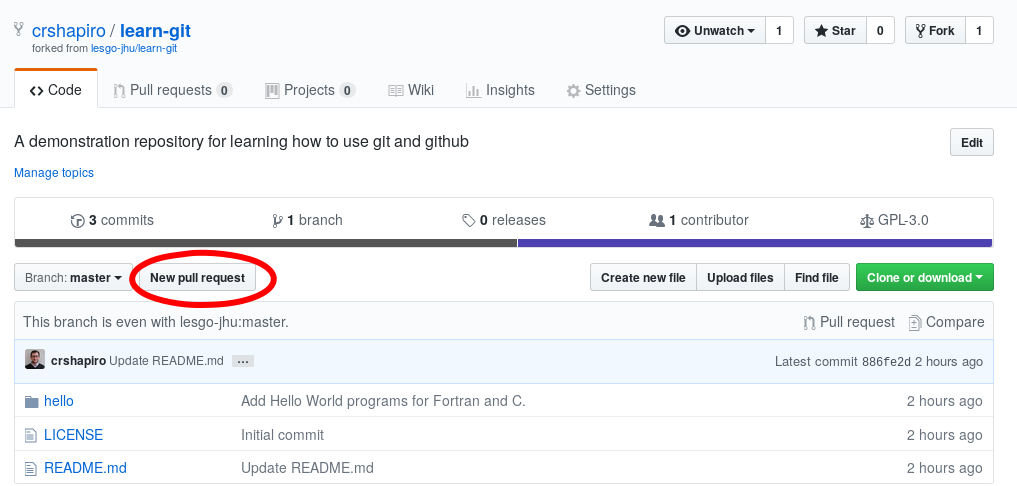
\includegraphics[width=\textwidth]{pull1.png}
\end{figure*}\\
Your changes will now show up as a pull request on the official repository waiting for approval from the maintainers.
\begin{figure*}[h!]
\centering
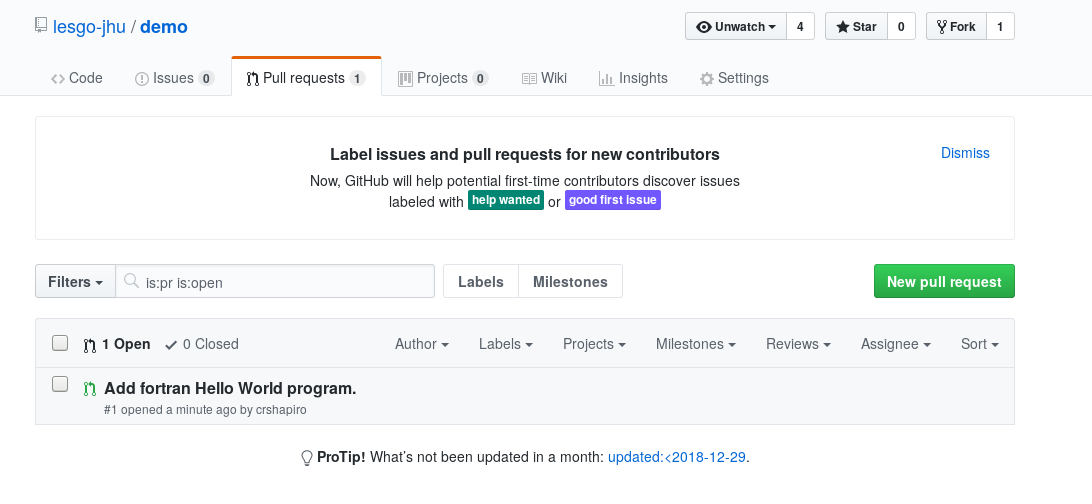
\includegraphics[width=\textwidth]{pull2.png}
\end{figure*}

\pagebreak
\item Now, you need to update origin to be even with the changes in upstream
\begin{lstlisting}
git fetch upstream
git rebase upstream/master
git push -f
\end{lstlisting}

\end{enumerate}

\section{Other important features}
\begin{itemize}
\item Branching. Check out \href{https://www.atlassian.com/git/tutorials/using-branches}{https://www.atlassian.com/git/tutorials/using-branches}
\item Merging. Check out \href{https://www.atlassian.com/git/tutorials/using-branches/git-merge}{https://www.atlassian.com/git/tutorials/using-branches/git-merge}
\item Merging vs. rebasing. Checkout: \href{https://www.atlassian.com/git/tutorials/merging-vs-rebasing}{https://www.atlassian.com/git/tutorials/merging-vs-rebasing}
\end{itemize}





\end{document}